\section{Evaluation}
\label{sec:evaluation}

This section discusses the behaviour of our algorithm in the real
world.

Both for testing and for performance evaluation, we require a test
suite. We started with a carefully crafted, manually produced, suite
of valid and invalid tests. This test suite was constructed by
gathering pairs of types that emerged from examples we have studied
and from programs we have written in FreeST, the programming language
for context-free session
types~\cite{almeida.etal_freest-functional-language}.
% This suite comprised of a total os 169 valid and invalid tests.  The
% primary purpose of this preliminary evaluation step was to confirm
% the algorithm would be able to handle manual examples that we knew
% would emerge from real programs and examples. The algorithm
% succeeded in evaluating all the tests in due time.
The tests produced by this method are, on the one hand, small, and, on
the other hand, lacking diversity.

We then turned our attention to the automatic generation of test
cases. Generating pairs of arbitrary (well-formed) types that share no
variables is simple. The difficulty lies in deciding whether two such
types, independently generated, are bisimilar. Even if an oracle could
be identified, the probability that a randomly generated pair of types
turns out to be equivalent would be extremely low. Instead, we proceed
by generating arbitrary pairs of types that are bisimilar by
construction. Theorem~\ref{thm:axioms} naturally induces an algorithm:
given a natural number $n$ (the size of the pair), arbitrarily select
for the base case ($n=0$) one of the pairs in item 1 of the theorem
and for the recursive case ($n\ge1$) one of the pairs in 2--12 items.

\begin{theorem}[Properties of type equivalence]
\label{thm:axioms}
  \begin{enumerate}
    % Congruence
  \item $\skipk \TypeEquiv \skipk$,  $\sharp B \TypeEquiv \sharp B$, and
    $X \TypeEquiv X$;
  \item $S;T \TypeEquiv U;V$ if $S \TypeEquiv U$ and $T \TypeEquiv V$;
  \item $\mu X.S \TypeEquiv \mu X.T$ if $S \TypeEquiv T$;
  \item $\star\{\ell_i\colon S_i\}_{i\in I}\TypeEquiv
    \star\{\ell_i\colon T_i\}_{i\in I}$ if $(S \TypeEquiv T)_{i\in
      I}$;
    % Laws for sequential composition
  \item $S\TypeEquiv T;\skipk$ and $S\TypeEquiv \skipk;T$ if $S \TypeEquiv T$;
  \item $\star\{\ell_i\colon S_i\}_{i\in I};U\TypeEquiv
    \star\{\ell_i\colon T_i;V\}_{i\in I}$ if $(S_i \TypeEquiv T_i)_{i\in
      I}$ and $U \TypeEquiv V$;
  \item $T \TypeEquiv S$ if $S \TypeEquiv T$;
  \item $R;(S;T) \TypeEquiv (U;V);W$ if $R \TypeEquiv U$, $S \TypeEquiv V$, and $T\TypeEquiv W$;
    % Laws for mu-types
  \item
    $\mu X.\mu Y.S \TypeEquiv \mu X.\subs XYT \TypeEquiv \mu Y.\subs
    YXT$ if $S \TypeEquiv T$;
  \item $\mu X.S \TypeEquiv T$ if $S \TypeEquiv T$ and $x\notin\free(S)$;
  \item $\subs UXS\TypeEquiv \subs VXT$  if $S \TypeEquiv T$ and $U \TypeEquiv V$;
  \item $\mu X.S \TypeEquiv \subs{\mu X.T}{X}T$ if $S \TypeEquiv T$.
  \end{enumerate}
\end{theorem}
%
\begin{proof}
  1--3: Bisimulation is a congruence. 4--12: Thiemann and
  Vasconcelos~\cite{thiemann2016context} exhibit the appropriate
  bisimulations.
\end{proof}

For evaluating the algorithm on non-bisimilar pairs we independently
generate two types, run function $\BisimT$ on them, and discard the
data collected in the rare event that the pair turns out to be
bisimilar.
%
For testing, however, we rely on manually crafted tests, for a
solution based on anti-axioms does not work: bisimulation for
context-free session types is such that there are types $S \not\bisim
T$ such that $\mu X.S \bisim \mu X.T$ (just think of $!\intk;X;X$
and $!\intk;X$).

We used QuickCheck~\cite{DBLP:conf/icfp/ClaessenH00} generate the test
suite. That for bisimilar pairs (constructed based on
Theorem~\ref{thm:axioms}) comprises 2000 pairs, featuring types with a
number of nodes (in the syntax tree) ranging from 1 to 35751. The test
suite for non-bisimilar pairs (constructed by independently generating
two types and verifying they were not equivalent) includes 2000
pairs with a number of nodes ranging from 1 to 387.
%
The slowest negative test takes under 775Mb of RAM to execute.

\begin{figure}[t]
    \centering
    \subfloat[Distribution of the execution time]{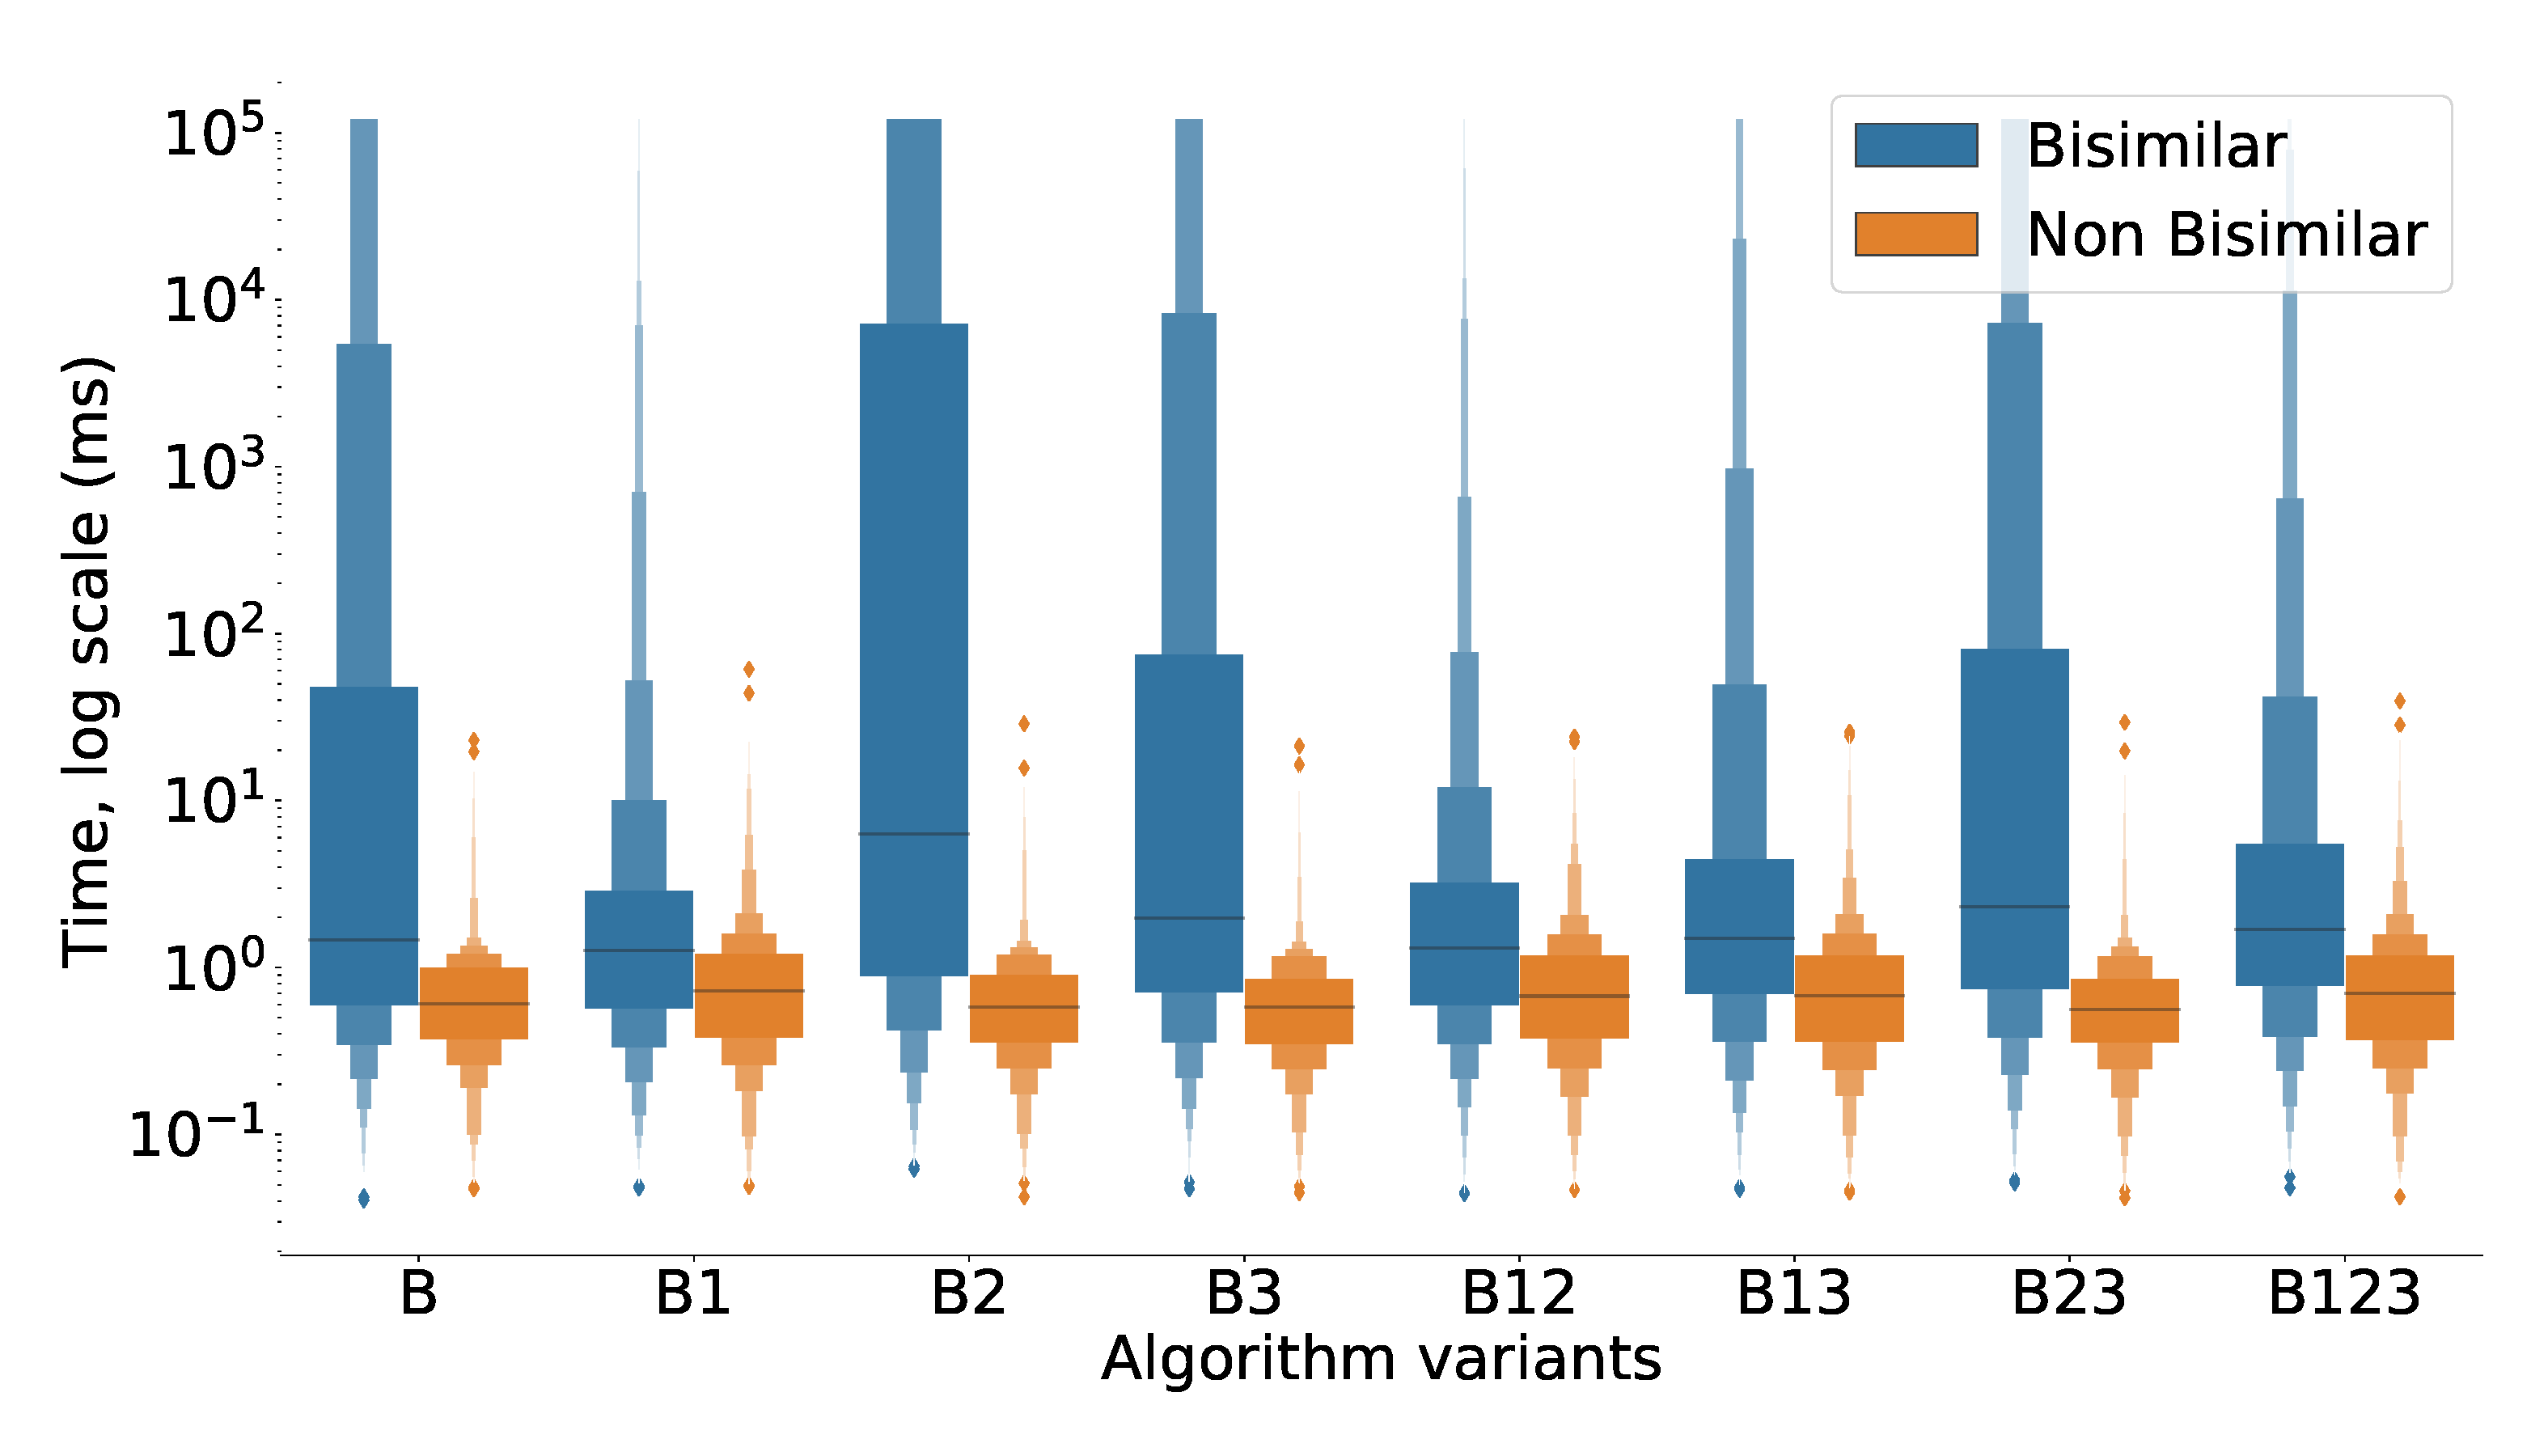
\includegraphics[height=.5\textwidth]{img/distribution_boxplot}}%
    \subfloat[Execution time per number of nodes]{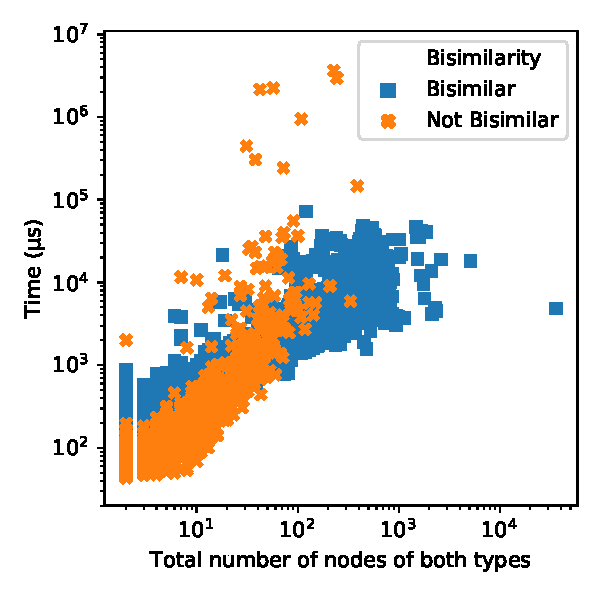
\includegraphics[height=.5\textwidth]{img/nodes_time_B0}}%
    \caption{The test suite composed by equivalent pairs of types is represented in blue and the
    test suite with non-equivalent pairs of types is represented in orange. Time 
    in microseconds, $\mu s$. Both scales are logarithmic.\\
    (a) Distribution of execution time of function $\BisimT$ for both test suites.\\
    (b) Distribution of execution time of function $\BisimT$ per total number of nodes 
    in the abstract syntax trees of the types.}%
    \label{fig:results}%
\end{figure}

%\begin{figure}[h]
%\centering
%	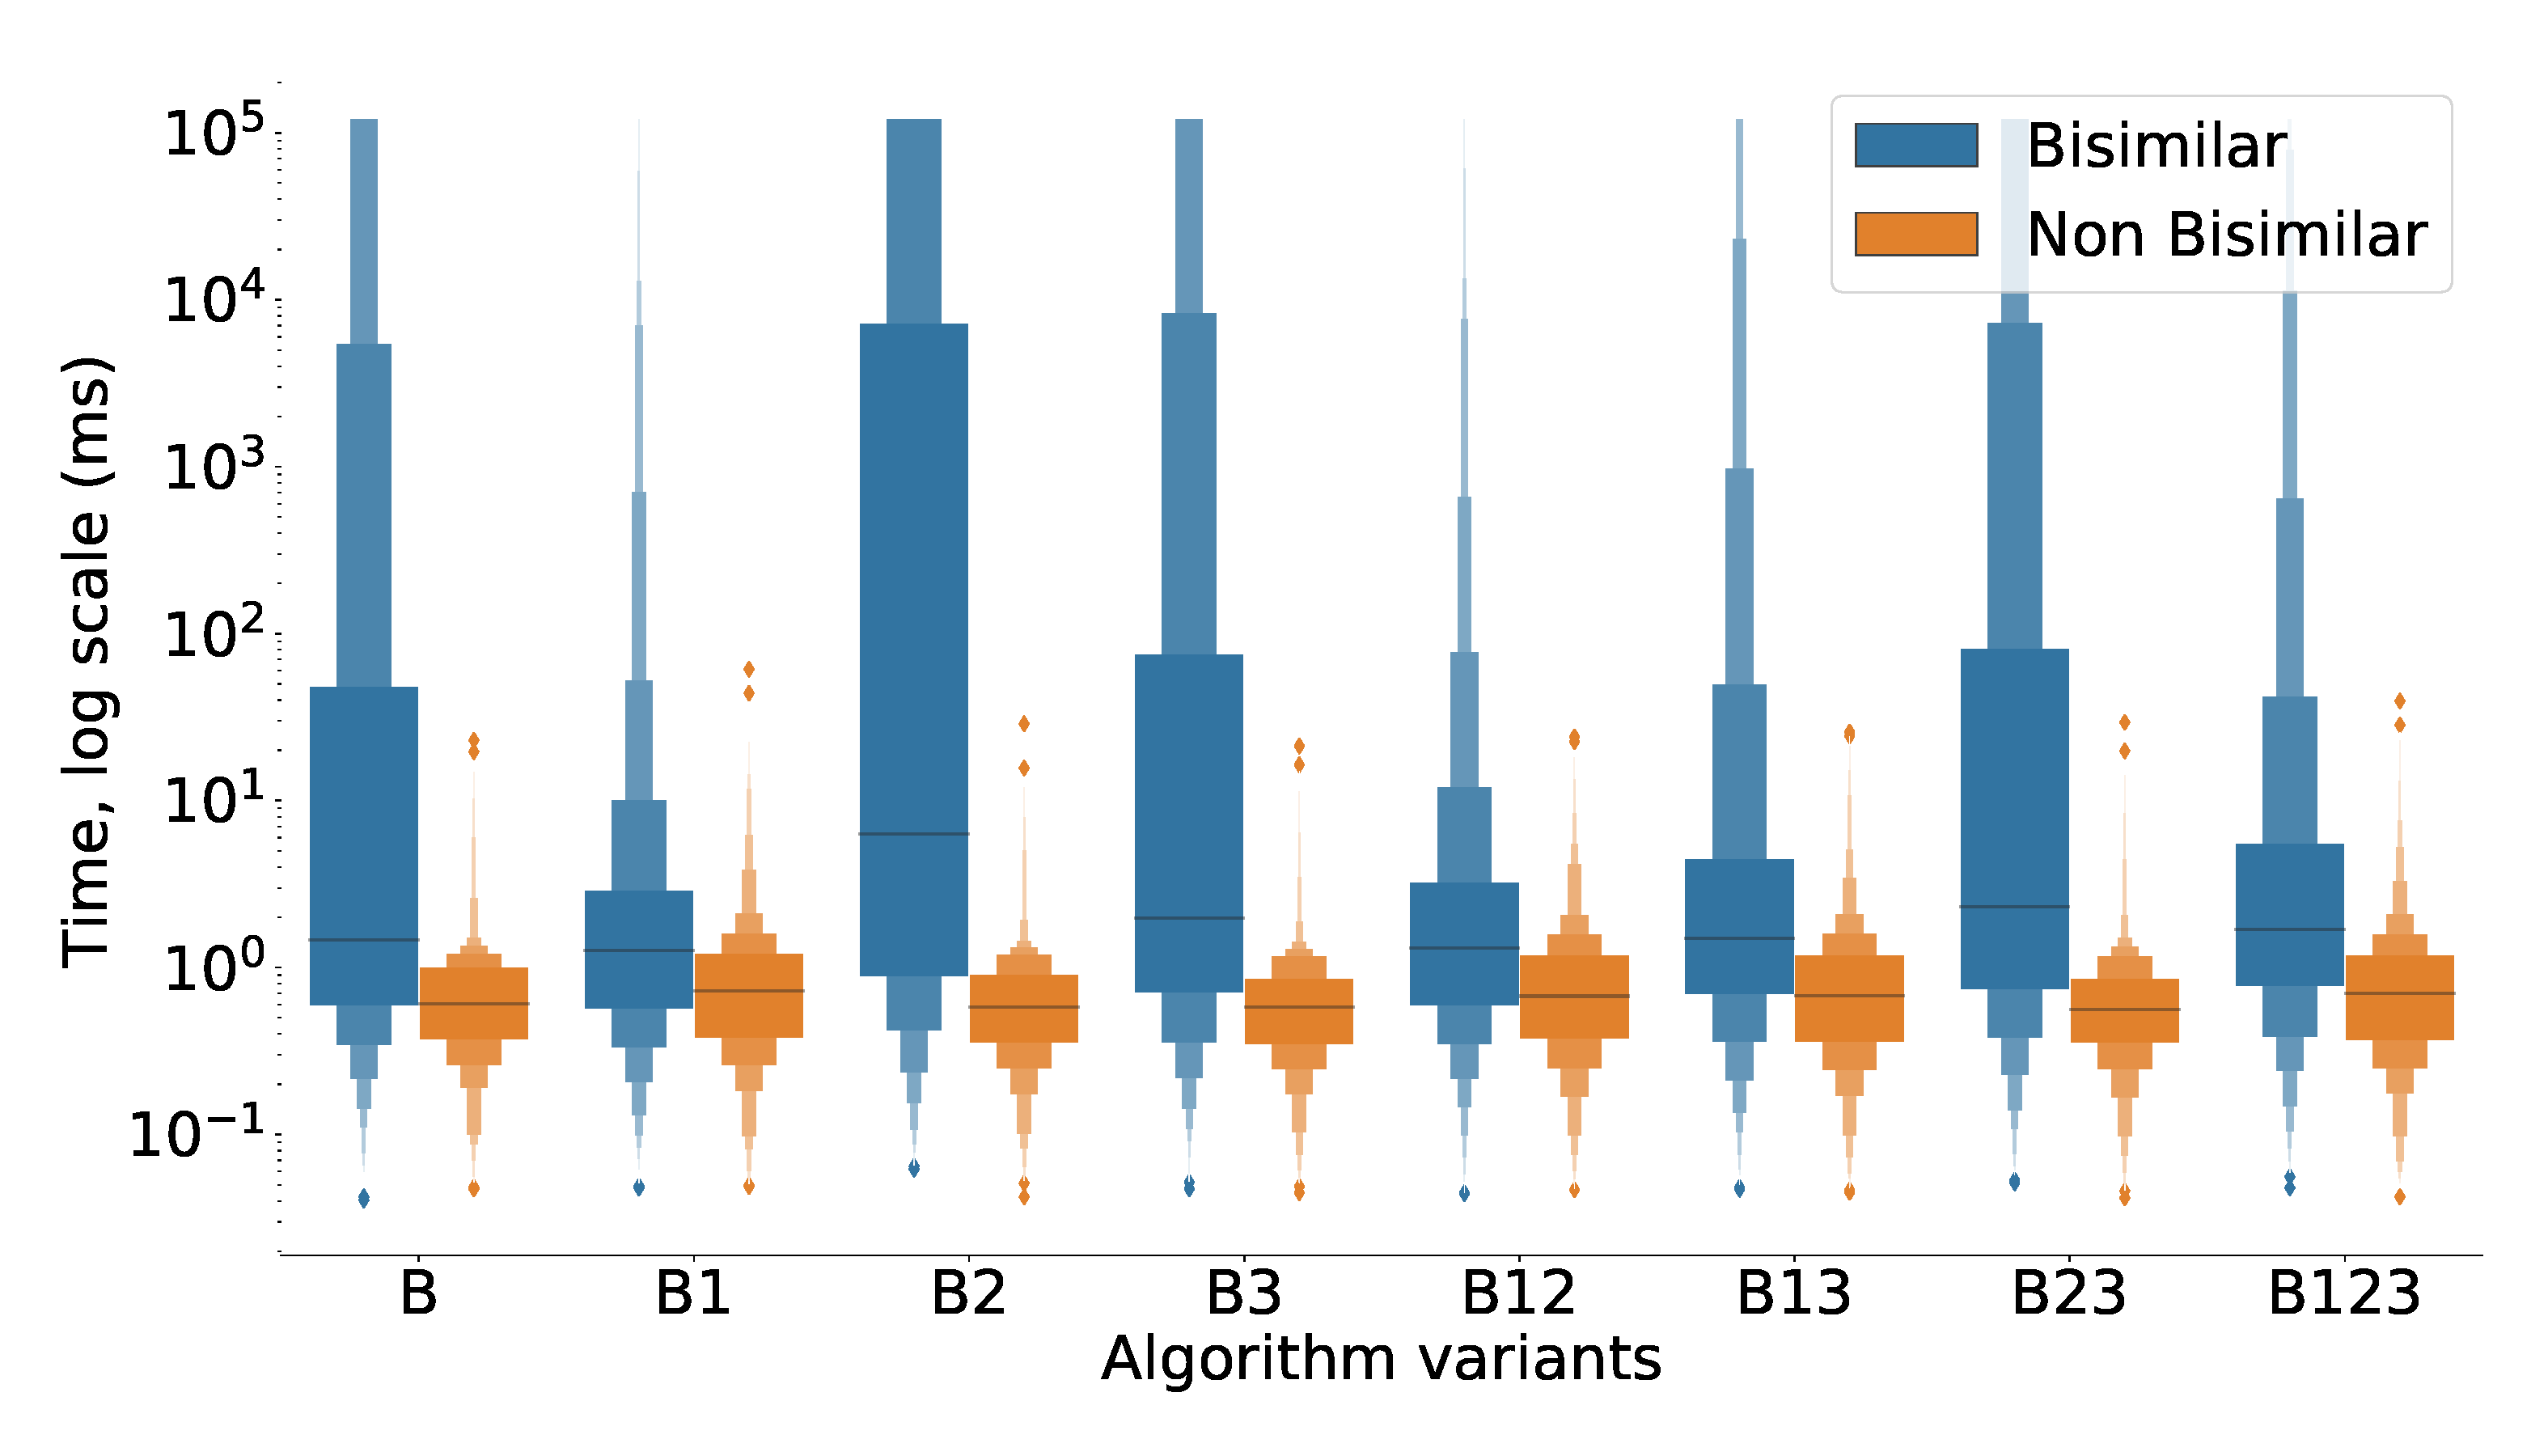
\includegraphics[height=6cm]{img/distribution_boxplot}	\hspace*{2mm}
%	\caption{Distribution of execution time of function $\BisimT$ for the 
%	test suite with equivalent pairs of types (blue, at the top) and for the 
%	test suite with non-equivalent pairs of types (orange, at the bottom).
%	Time is represented in microseconds, $\mu s$.}
%	\label{fig:run_times}
%\end{figure}
%\begin{figure}[h]
%\centering
%	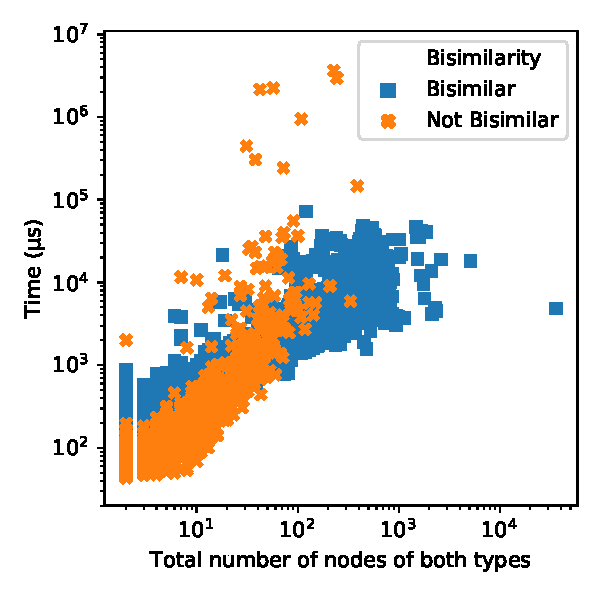
\includegraphics[height=6cm]{img/nodes_time_B0}
%	\caption{Distribution of execution time per total number of nodes for
%	equivalent and non-equivalent pairs of types (represented by blue and
%	orange, respectively). Time is represented in microseconds, $\mu s$.}
%	\label{fig:nodes_vs_time}
%\end{figure}

We implemented the algorithm described by the function $\BisimT$ in
300 lines of Haskell and used the Glasgow Haskell Compiler (version
8.6.5), provided by the docker image
\texttt{fpco/stack-build}. Evaluation was conducted on a machine with
an Intel Xeon X5670 at 2.93GHz and 24 GB of RAM.
%
Figure~\ref{fig:results} (a) depicts the distribution of the execution
times (in $\mu s$) for both test suites. All tests completed in less
than 1 minute. We see that the majority of the tests terminate within
0.01s.  The figure also shows that deciding equivalence negatively is
slightly faster than deciding it positively.

%\begin{figure}[h]
%	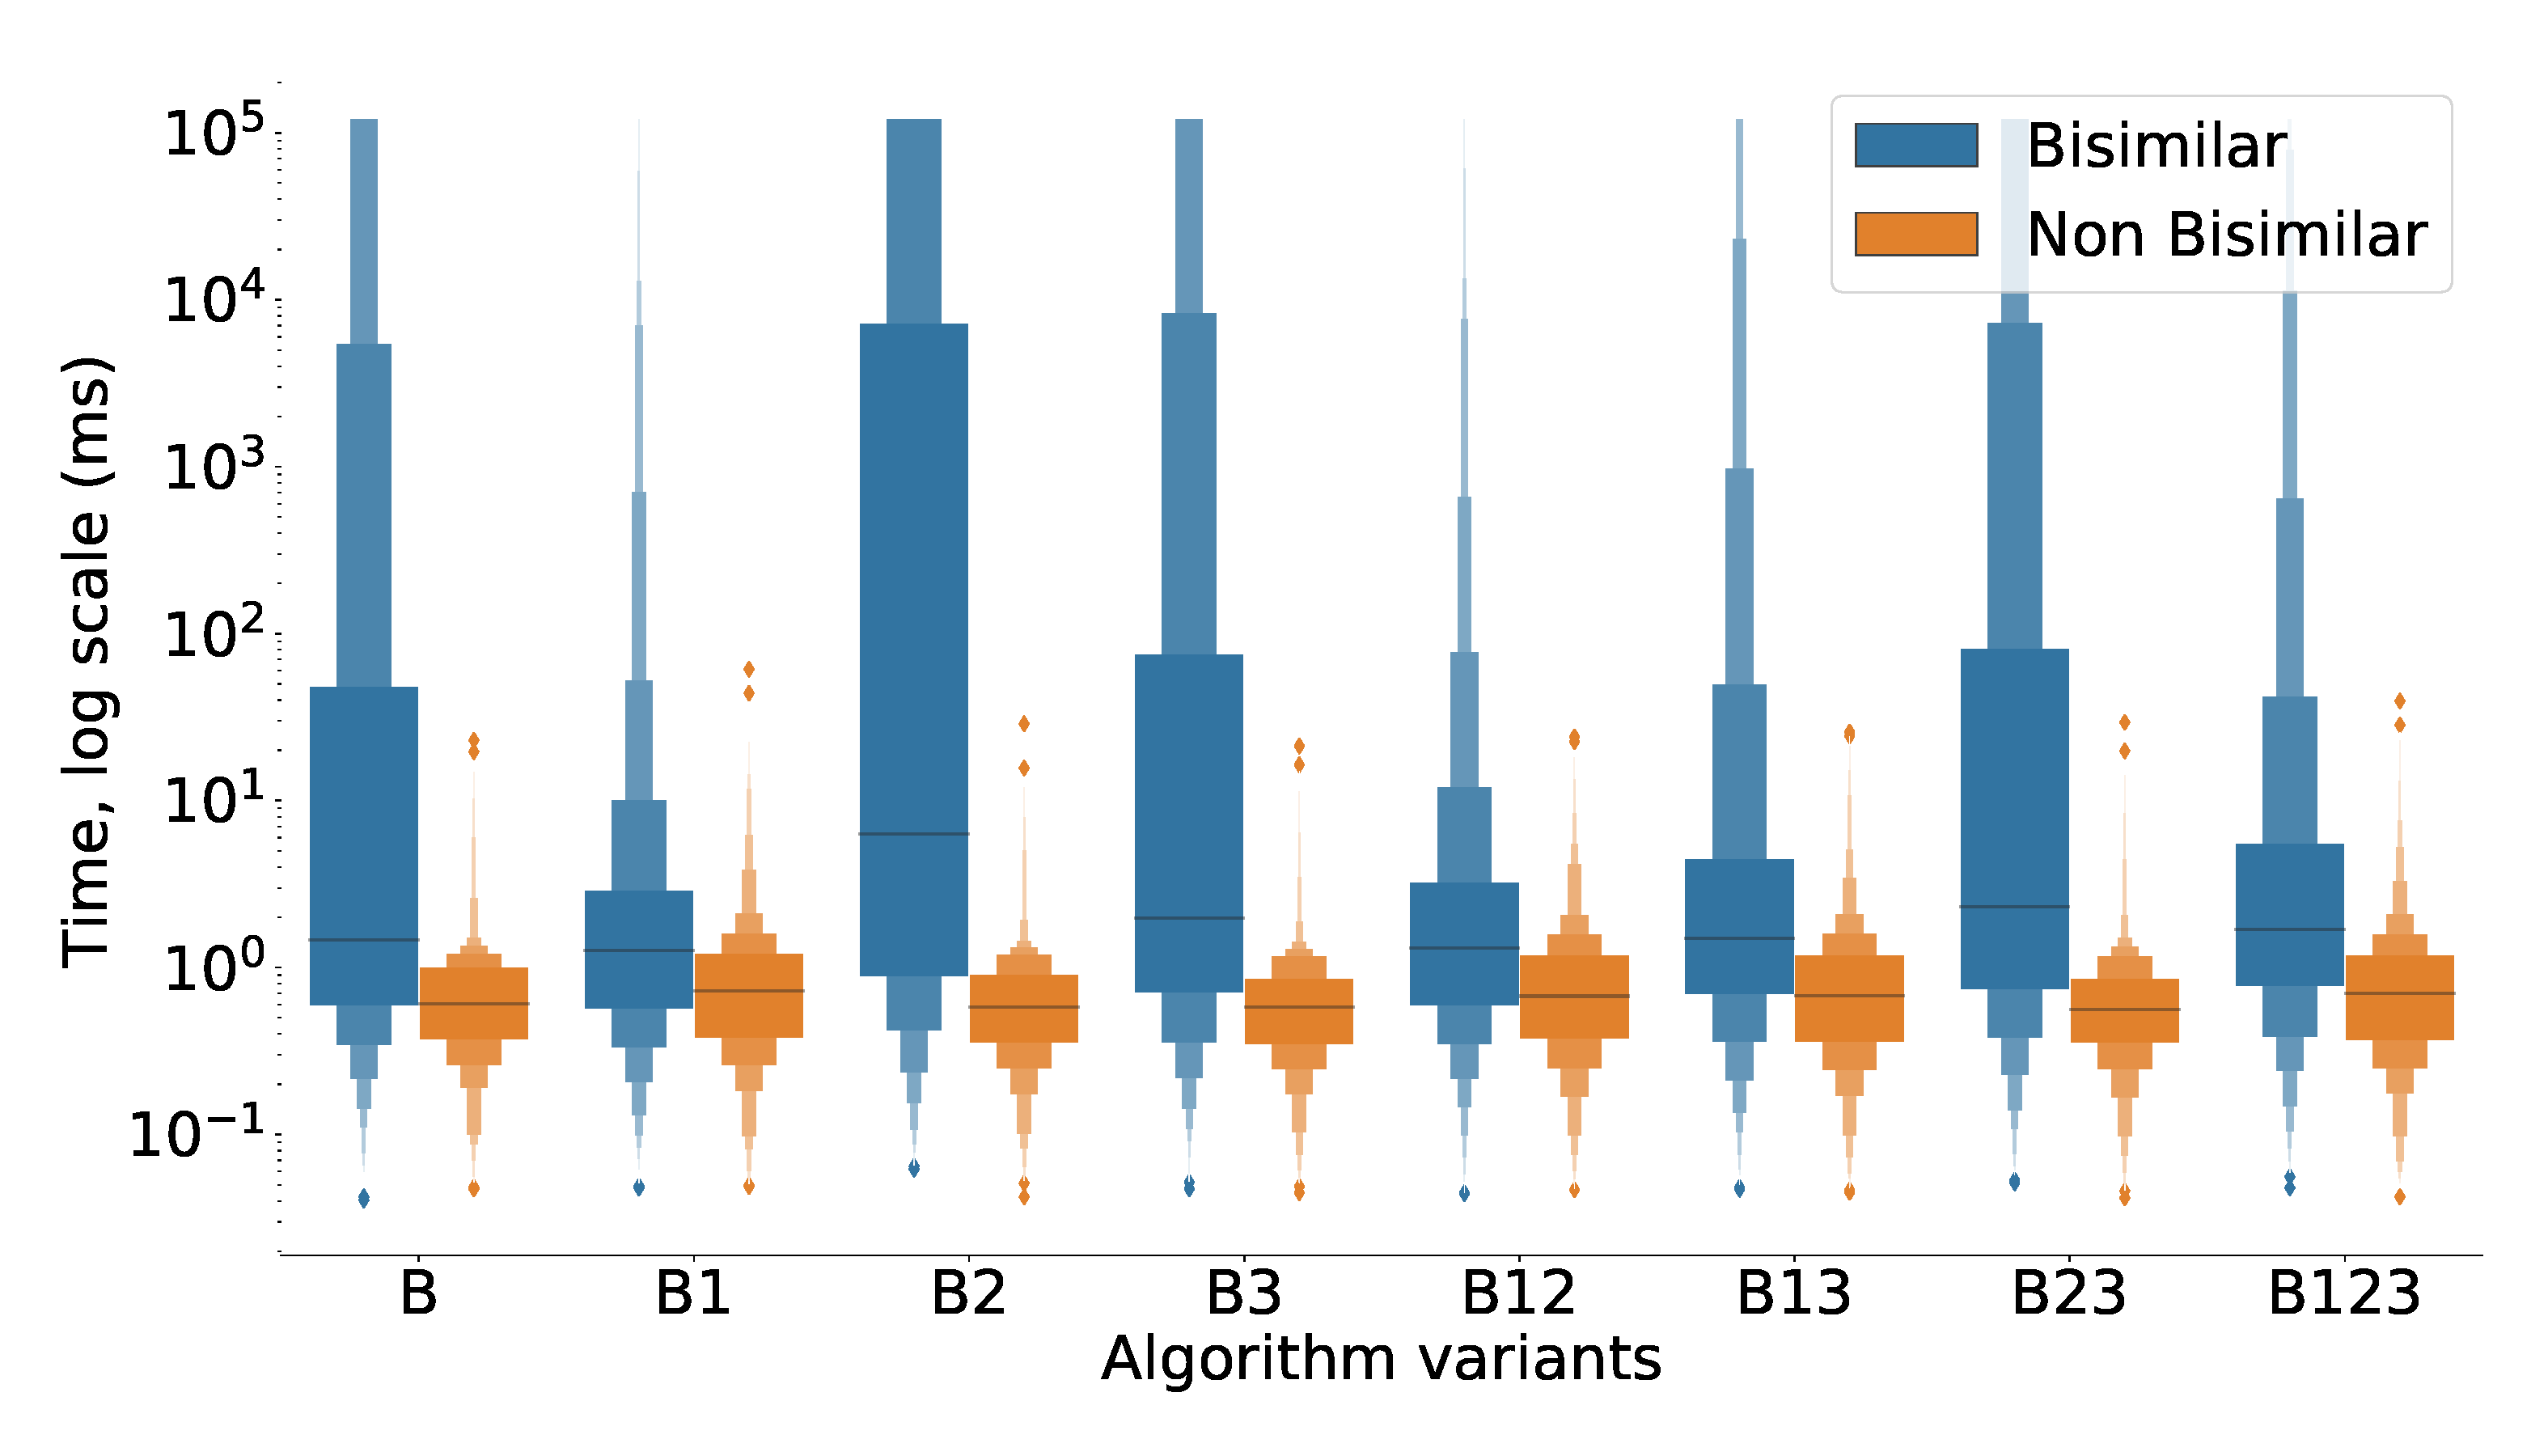
\includegraphics[height=6cm]{img/distribution_boxplot}	\hspace*{2mm}
%	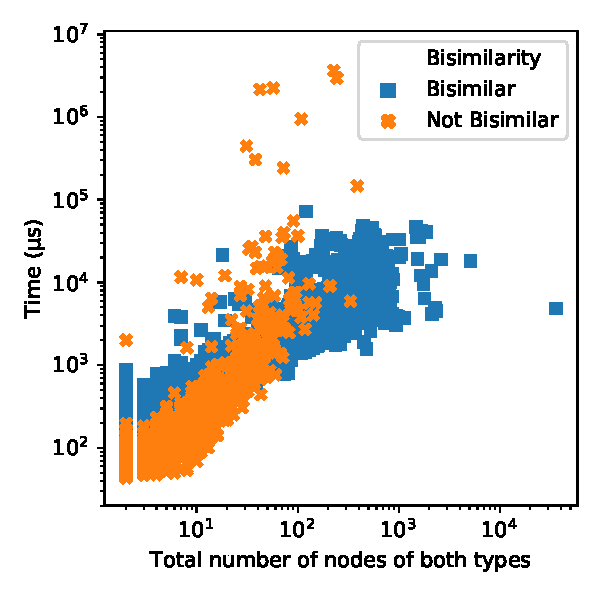
\includegraphics[height=6cm]{img/nodes_time_B0}
%	\caption{Distribution of execution time of function $\BisimT$ (on the left) and distribution of execution time per total number of nodes of both types (on the right).}
%	\label{fig:results}
%\end{figure}


Figure~\ref{fig:results} (b) represents the distribution of execution
time per total number of nodes in the abstract syntax trees of the
types. For the positive tests, we observe a linear increase in the
runtime, whereas for the negative tests what seems to be the execution
time increases exponentially.  We suspect that if we had carried out
tests with a larger number of nodes, we would also have had observed
an exponential growth in the execution time.

Although the runtime of the algorithm is good enough for a compiler,
we identified a few potential optimisations and analysed their impact
on the execution time of function $\BisimT$. We implemented the
following variations: i) eliminating redundant productions in the
grammar, ii) using a double-ended queue where promising children are
prepended rather than appended, iii) adding a filter rule to
simplification stage that removes hopeless pairs from nodes, and iv)
iterating the simplification stage until a fixed point is reached.
%
Running the test suite discussed above in these variants, alone and
in different combinations, we found no decrease in the runtime.

% Once the improvement proposals were established, we benchmarked the
% algorithm on a test suite of carefully crafted pairs of types
% based on cases observed when using the compiler where the algorithm is
% used~\cite{almeida.etal_freest-functional-language}. These
% tests comprise valid and invalid equivalences, for a total of 154
% tests. We have profiled our program for the time and memory allocated
% during the tests. For this purpose, we have used GHC's profiling
% feature, that maintains a cost-centre stack to keep track of the
% incurred costs. The results are depicted in
% Figure~\ref{fig:results}.

% \begin{figure}[h]
% 	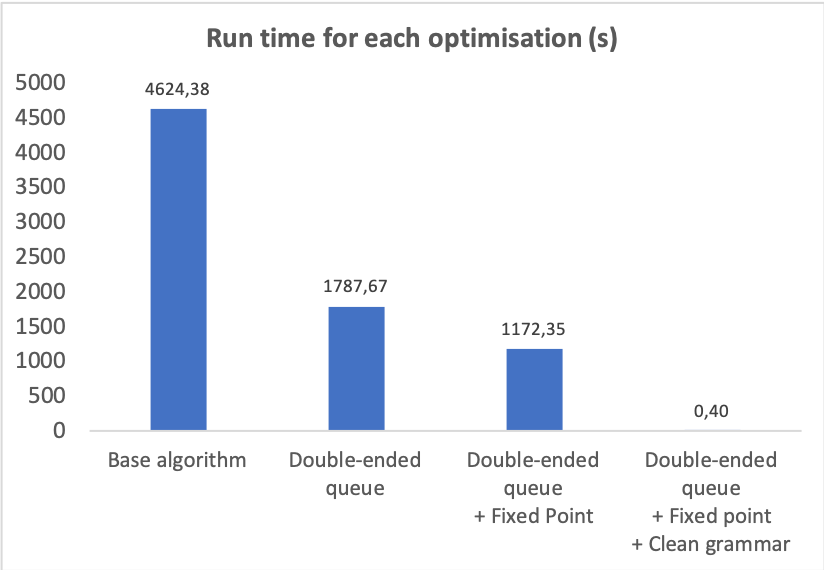
\includegraphics[height=4cm]{img/run_time}	\hspace*{2mm}
% 	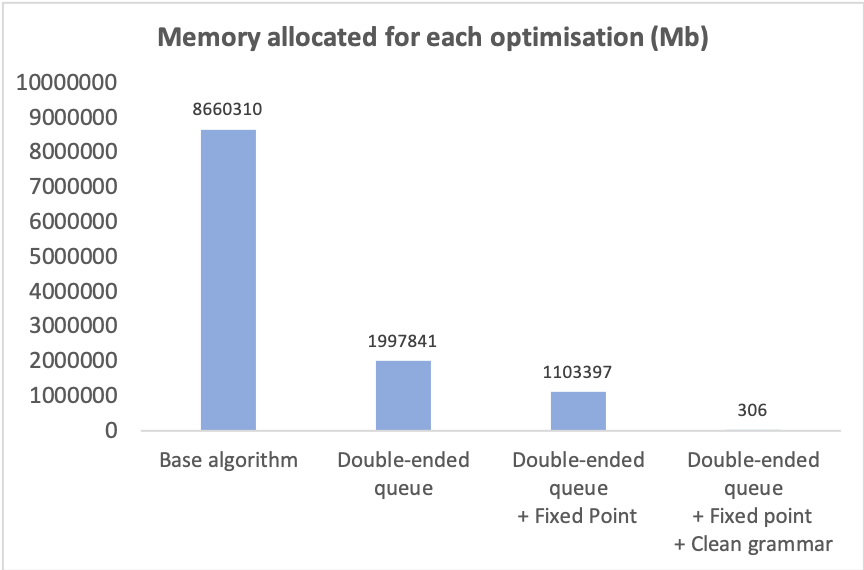
\includegraphics[height=4cm]{img/memory_alloc}
% 	\caption{Test results: running times (on the left) and
% 	memory allocated (on the right) checking the equivalence
% 	of context-free session types in 154 tests.}
% 	\label{fig:results}
% \end{figure}

% For the base algorithm, proposed in Listing~\ref{lst:algorithm}, we
% obtained a running time of about 4624 seconds and
% 8,660,309 Mb memory allocated. From the moment we introduced the
% optimizations the results improved remarkably:
% implementing a double-ended queue we reduced the running time to 1788
% seconds and the allocated memory to 1,997,841 Mb, by also
% iterating the
% simplification phase in the search for a fixed point we decreased these values
% to a running time of 1172 seconds and
% allocated memory of 1,103,397 Mb. The
% combination of these enhancements with the clean grammar generation
% exhibit an improvement in more than 1,000,000\% from the base case,
% achieving a running time of 0.4 seconds and 306 Mb
% of memory allocated.

% %iterating the
% %simplification phase in the search for a fixed point allowed to reduce
% %the running time to 110.35 seconds and the memory allocated to 164,745
% %Mb, whereas the implementation of the double-ended queue allowed to
% %reduce the running time to 18.45 seconds and the allocated memory to
% %29,298. The combination of both exhibit an improvement on more than
% %1,000,000\% from the base case, achieving an average of 0.04
% %seconds for the running time and 62 Mb of allocated memory.

% We should also highlight that, we run example~\eqref{ex:chaotic}
% with the improved algorithm, in a battery of 100 runs, and obtained an
% average running time of 0.008 seconds.

% The heuristic we proposed actually circumvents the exponential complexity
% inherent to the expansion tree, thus allowing to obtain running times that
% are manifestly small and to use this algorithm as an integral
% part of a compiler, as we had intended from the beginning.

%%% Local Variables:
%%% mode: latex
%%% TeX-master: "main"
%%% End:
